\chapter{绪论}
\section{课题来源}
本课题来自国家科技重大专项“极大规模集成电路制造装备及成套工艺”(02专项)28nm节点浸没式光刻机产品研发项目子课题七“浸没光刻机亚纳米精度运动控制技术研究”(课题编号2017ZX02101007)。
\section{研究背景与意义}
扫描投影光刻机是半导体制造领域地位最为重要、技术难度最大、复杂程度最高的设备,也是目前芯片特征尺寸逐渐缩小,功能不断强大的有力保障。随着摩尔定律和后摩尔时代的发展,芯片的集成度将仍保持指数级增长,3$\sim$5纳米工艺节点呼之欲出。这种必然的趋势对整个集成电路产业链,包括设计、制造、封装和测试均提出了更高的要求,尤其是芯片制造领域,意味着未来必然迎来各种极大规模集成电路制造设备与工艺的升级换代。

集成电路的快速发展得益于光刻工艺的不断进步。在光刻工艺中,光刻机是决定性的设备,其必须同时满足芯片制造的关键尺寸、套刻精度和产率三大核心要求。如图\ref{光刻原理图1}所示,光刻机主要由光源及其控制系统、运动台及其控制系统以及环境控制系统等构成。整个光刻控制系统可以说是该设备的“大脑”,必须时刻维持高速、精准的控制,其作用主要是对硅片以及印有电路图形的掩模版进行超高精度、超高速度的操作,同时实现多自由度的空间相对运动,保证设计好的电路图形可以在亚纳米精度准确无误地曝光到硅片上,完成图形的转移。从实际需求考虑,光刻机控制技术的挑战主要集中在三个方面\cite{butler2011position}:1)小尺寸。现代集成电路芯片的特征尺寸逐渐缩小,已达到纳米级甚至亚纳米级,要保证电路图形精准地刻画在晶圆上,扫描曝光过程中允许的位置误差只有几纳米甚至不到1纳米,仅为特征尺寸的一小部分;2)高产率。光刻机用于大规模批量生产线,对产率的要求很高,通常每小时的产量为175片以上;3)高鲁棒性和可靠性。实际工业生产线上,保证机器持续稳定地工作是必然的追求,这与测量系统、环境调节和控制策略都有很大关系。

从运动台及其控制角度来看,曝光成像过程要在高速运动中完成,其扫描和定位精度直接影响曝光成像质量,包括成像精度和套刻精度,因此对光刻机运动系统的扫描和定位精度要求达到纳米级精度甚至亚纳米级精度。另一方面,高产率的需求要求运动系统具有高速高加速的特性,而高速高加速引起的振动会导致精度恶化、整定时间变长,从而导致产率下降。可以看出,高速度、高加速度、高精度以及高产率之间是相互矛盾的,需要采用额外的控制措施使得相互制约的性能指标都达到一个较为理想的值,这是一个非常具有挑战的工作。

\begin{figure}[!t]
	\centering
	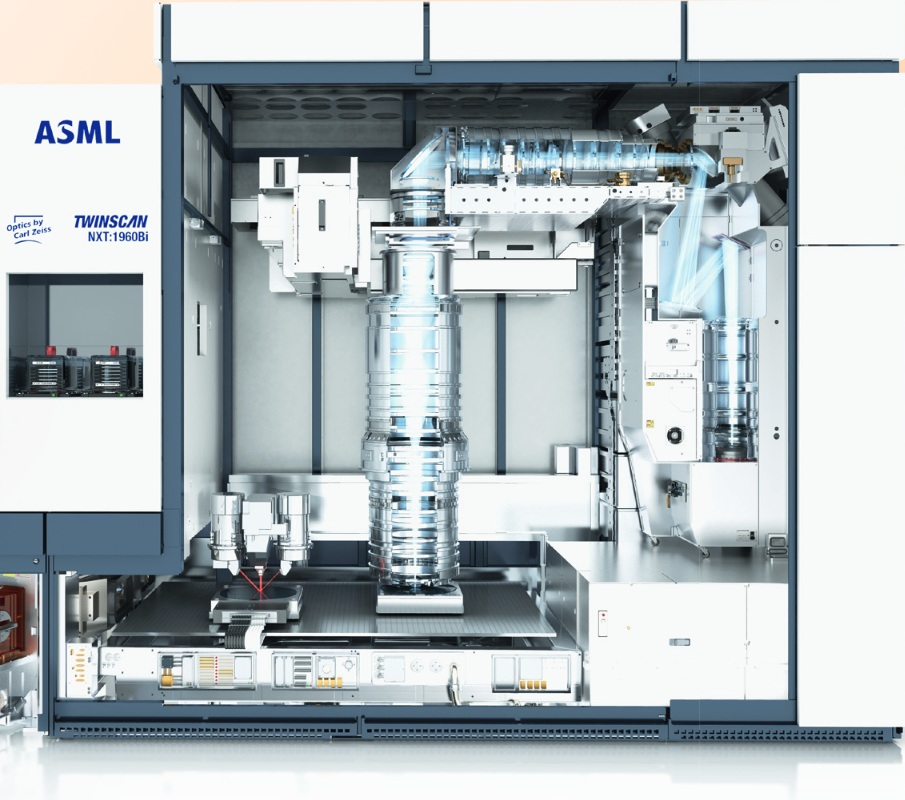
\includegraphics[width=12cm]{figures/光刻原理图2}
	\caption{ASML扫描投影光刻机}
	\label{光刻原理图1}
\end{figure}
\begin{comment}
在扫描光刻控制系统领域,大部分还是使用闭环PID反馈控制器,PID 控制器的优点是明显的:简单好用,P,I,D 各项物理意义明确,稍有研究即可对其进行参数调试。基于PID解耦控制技术的传统工件台运动控制方法虽然已经取得了较好的效果[2-4],而且现在很多中低端光刻控制系统中仍然在使用传统PID控制方法,但是传统PID控制方法存在的一些问题限制了扫描光刻系统性能的进一步提升。首先,PID方法仅能解决单输入-单输出(SISO)控制问题。虽然现在运用解耦控制技术,可以将多输入-多输出(MIMO)通过解耦转换为单输入-单输出(SISO)控制问题。但实际效果很大程度上取决于解耦过程以及系统各变量之间的复杂关系,另外需要考虑系统各变量自身的稳定性,这些要求在工业环境中极为苛刻,很难保证完全解耦且系统各变量自身不随环境变化而变化。其次,传统PID方法缺乏对非线性因素的考虑,而扫描光刻系统的工件台控制存在非线性因素的影响,此外由于负载的变化、外界的扰动以及设备自身的磨损等因素引起的模型不确定性和一些未建摸特性都会影响传统PID控制系统的鲁棒性和稳定性。最后,PID 参数本身整定困难,而且一组参数一般只适用于一种工况,对时变的,动态的,非线性的,复杂的系统适应性差,而且在系统快速性和稳定性上难以同时兼顾。在这种情况下,针对原来系统模型设计的PID控制器不再合理,甚至失效,以至无法达到理想的控制效果。因此,对PID控制器的参数整定的研究具有重要的意义。
\end{comment}


光刻机运动台包括工件台和掩模台,其高速度和高加速度基本上都是由精密直线运动平台作为执行机构产生\cite{butler2011position},因此,要平衡高速度、高加速度、高精度以及高产率等性能要求,对精密直线运动平台进行高性能运动控制是重要突破点之一。精密直线运动平台经历了机械导轨、气浮导轨以及磁浮导轨的发展,但是不变的是执行机构大都是基于永磁同步直线电机(Permanent Magnet Synchronous Linear Motors, PMLSMs)或其变种,因此本文将基于PMLSMs的精密直线运动平台作为研究对象。如图\ref{直线电机结构}所示,相比于传统基于旋转电机的直线运动平台,PMLSMs摆脱了中间传动机制的限制,因而更适用于高速、高加速定位系统,然而,由于省略了中间传动机构,定位力、线缆力、纹波扰动以及模型参数摄动和外部扰动等不确定性因素将直接影响PMLSMs的位置跟踪性能\cite{wang2015detent}。因此,如何提高系统的扰动抑制能力成为实现PMLSMs高性能控制的关键\cite{yang2018investigation}。

PMLSMs的端部力和齿槽力合称为定位力,与电机的磁体结构有关,是一种不依赖于时间的扰动,只与PMLSMs动子运动的位置相关。线缆力也是一种位置依赖的扰动,其与位置的关系也呈现出典型的非线性特性\cite{yang2018integrated}。已经有很多经典模型被提出\cite{tan2002robust,chen2009modeling,wassink2005lpv},通过建模的方式能够在一定程度上消除定位力和线缆力对于PMLSMs位置跟踪性能的影响,但要进一步提高控制性能,还需要对定位力和线缆力的未建模部分以及纹波扰动、模型参数摄动、未知的外部扰动等时变的非线性扰动进行一定的补偿。
非线性扰动已经是影响工件台精度的主要原因之一。由于含有具有开关特性的鲁棒项,滑模控制能够有效地抑制非线性扰动\cite{heertjes2014self,li2016state}。自提出以来,滑模变结构控制已经拥有了非常成熟的一套理论体系\cite{young1999control},而且滑模控制方法简单易用,能够很自然地与自适应控制\cite{huang2008adaptive}、模糊控制\cite{tong2003fuzzy}以及神经网络控制\cite{qi2013adaptive}相结合,如今在精密运动控制领域也得到了广泛的应用。神经网络在处理非线性问题的时候,由于其对于非线性函数有着良好的拟合能力,且不需要具体的模型信息,因此对于补偿未知的时变扰动非常有优势。从实际应用的角度考虑,如果能够充分发挥滑模控制以及神经网络在非线性控制方面的优势,将非常有利于解决扫描光刻系统工件台控制面临的非线性影响因素带来的问题。
\begin{figure}[!t]
	\centering
	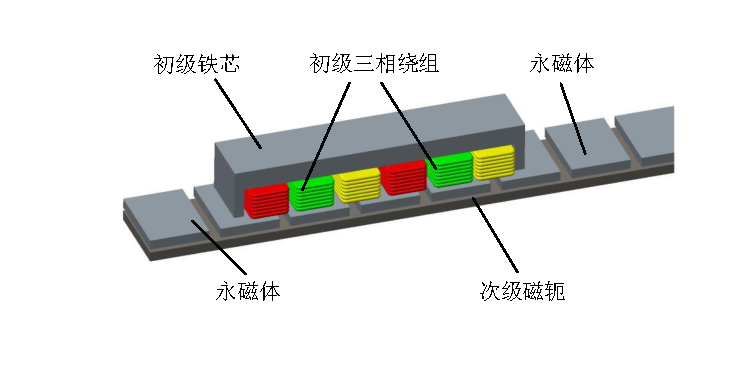
\includegraphics[width=12cm]{figures/直线电机结构图.pdf}
	\caption{永磁同步直线电机结构}
	\label{直线电机结构}
\end{figure}



本文通过对有铁芯PMLSMs动力学与扰动形式进行分析与建模,并结合递推最小二乘算法和神经网络的特性,对滑模变结构控制中的应用进行深入研究,旨在探索基于滑模控制的高性能运动控制方法来提高精密直线运动平台的位置跟踪性能和扰动抑制能力,以便其能够更广泛地应用于精密运动控制领域。
\section{精密直线运动平台控制方法研究现状及分析}
精密直线运动平台作为精密运动系统中的核心运动部件,广泛应用于集成电路制造、超精密伺服加工、纳米精度测量以及生物信息检测等领域\cite{董泽光2014精密气浮运动平台的建模}。在实际工程应用需求中,高速、高加速、高精度以及高稳定性是精密直线运动平台控制系统设计的主要目标。面临的控制方面的挑战主要来自于机械系统本身的谐振、定位力、测量噪声、参数摄动和电磁非线性以及外部非线性扰动等。在这些影响因素存在的情况下跟踪精度要达到纳米级,同时满足高产率的要求是一个极具挑战的工作。为了实现这些目标,国内外很多研究机构以及企业研发机构已经提出很多控制方法,这里对主要的几种控制方法做简要介绍。
\subsection{比例-积分-微分控制}
比例-积分-微分(Proportional-Integral-Derivative, PID)控制凭借其简单易用、物理意义明显等优势已经统治工程应用领域数十年,尤其是对于能够精确建模的应用对象,PID控制器能够实现良好的控制性能。但是随着技术的不断进步,对于精度和速度的极致追求使得传统的PID反馈控制方法面临了很多挑战。因此,现在的精密运动系统中常以改进的PID控制器作为反馈控制部分。Heertjes等人\cite{2009Performance}提出了一种N-PID,基于非线性滤波器,对经典PID控制方法进行了改进,从而提高光刻机工件台控制系统的位置跟踪性,并构建了李雅普诺夫函数,证明了其稳定性。Shin等人\cite{2011Anti}针对控制器输出饱和问题,提出了一种预测饱和稳态值的方法,让系统控制输出退出饱和时,将预测的稳态值引入积分环节并作为积分环节的初值,这样控制器的输出就能够很大程度上避免因饱和问题带来的超调大和整定时间长的问题,实验结果表明了所提方法在PID控制器存在输出饱和现象时拥有较好的控制性能。王学伦等人\cite{wang2011design}介绍了一种复合模糊免疫PID,用于PMLSMs的速度环,有效地提高了速度环的响应速度,通过自适应调节减小了速度环的误差。2014年,王辉和张段芹等\cite{王辉2014新型智能}提出了一种反向传播神经网络PID控制策略,网络的输出为PID参数,通过自适应的方法进行实时更新,有效地改善了基于永磁同步直线电机的调速系统的性能。2018年,一种基于扩张状态观测器的PID控制器被提出\cite{王文深2018基于},提高了气动机械手系统的定位精度和响应速度。2020年,一种基于粒子群优化的PID控制算法应用于微电子封装领域\cite{2020A},通过粒子群优化算法整定PID参数,改善了系统的控制指标。

PID控制器在运动控制领域的应用虽然仍旧非常普遍,但是随着跟踪精度要求越来越高,在超精密运动控制领域,单纯使用PID反馈控制器,实现高速、高精度控制有较大的挑战。因此,前馈控制与反馈控制相结合的方式引起了很多学者和工程师的关注。
\subsection{迭代学习控制}
迭代学习控制(Iterative Learning Control, ILC)是一种应用于重复参考轨迹的前馈控制方法,早期的期刊文献是1978年发表在日文期刊\cite{uchiyama1978formation},最初主要用于机械臂的重复轨迹控制中。ILC真正在学术界流行是1984年一系列文章\cite{1998Adaptive,kawamura1984iterative}发表之后,人们才认识到了ILC学习算法的重要价值。ILC作为一种前馈控制方式,不需要精确的数学模型,通过误差的迭代计算,即可学习到用于补偿扰动的补偿表,从而极大地提高系统的跟踪精度。Mishra等人\cite{mishra2010optimization}提出了一种基于优化约束的ILC设计方法,在执行器饱和约束的情况下采用跟踪误差的$L_2$范数作为评价指标,利用凸优化的思想设计得到ILC控制方法,提高了光刻机工件台位置跟踪性能,文章的主要贡献也是将数值优化的方法应用到了ILC的设计之中。Abidi等人\cite{abidi2010iterative}提出了一种基于时频域的ILC设计和分析的框架,比较了经典的P型、D型、D$^2$型和滤波器型的ILC的时频域特性,给出了采样时间与ILC收敛率之间的关系,对于ILC的设计提供了一种理论指引,最后还在压电平台上对于提出的设计框架进行了验证,仿真和实验结果都进一步表明所提设计准则的有效性。2007年,针对光刻机掩模台的一些非线性问题,Heertjes等人\cite{heertjes2007nonlinear}提出了一种非线性ILC,非线性主要体现在学习增益的设计中,在收敛速率和噪声抑制的平衡方面有了很大的改善。张等人\cite{zhang2018data}提出了一种局部动态线性化的方法被应用于针对非线性系统的自适应迭代学习控制系统设计中,整个系统的设计不依赖于模型信息,完全依赖于系统输入输出的数据,最后通过仿真验证了这种线性化的技术有益于数据驱动的ILC在非线性系统中的应用。Hao等人\cite{hao2020extended}针对工业批处理过程中的时变的不确定和外部扰动问题,提出了一种时域和迭代域相结合的ILC,这种ILC方法采用了双环结构,内环用基于扩张状态观测的反馈控制结构保证位置跟踪时间上的鲁棒性,外环采用P型ILC保证批处理过程的收敛性,还基于线性矩阵不等式保证了整个控制系统的输出是有界的。ILC在重复扰动占主导地位的控制系统中能够保证很好的控制性能,但是当系统中的非重复扰动占主导时,往往ILC控制性能会变差\cite{mishra2007precision}。为了解决基于采样数据的迭代学习控制在非重复扰动存在情况下的收敛性问题,池荣虎等人\cite{chi2020convergence}提出了一种新的分析方法,结合数学归纳法与收缩映射原理证明了系统变量的有界收敛性,并证明了当迭代变化的不确定性消失的情况下,系统跟踪误差能够收敛到一个较小的边界,这些结构都能够放松ILC限制性的重复条件。

但是在实际工业应用环境中,系统模型参数可能会出现摄动现象,即模型参数会随着时间有微小的变化,这种情况下,ILC作为一种典型的前馈控制方法,对于模型参数的变化非常敏感,进而会影响系统的跟踪精度。针对这种模型参数摄动等需要在线调节和控制的问题,人们对自适应控制寄予了更多期待。
\subsection{自适应控制}
自适应控制主要用来应对系统不确定性随时间或空间变化的情况,控制器能够根据系统状态的变化实时地进行调整以提高系统的跟踪性能和扰动抑制能力。2012年,Butler\cite{butler2012adaptive}针对光刻机工件台中位置依赖的扰动,提出了一种自适应前馈的方式,通过在线调整系统前馈控制器参数提高了系统的位置跟踪精度并缩短了系统曝光前的整定时间,该文通过很多的实际工程问题验证了高阶前馈控制器能够比仅采用加速度前馈更有效地减小位置跟踪的误差峰值。针对PMLSMs系统存在的周期性的扰动,一种新型的自适应扰动补偿策略被提出\cite{cho2014high},主要用来减小重复性的扰动,这一新型的自适应扰动观测器不依赖于扰动的模型,在每个时间周期内通过更新周期的自适应律进一步地削弱扰动带来的影响。张等人\cite{zhang2019force}将模型参考自适应(Model Reference Adaptive Control, MRAC)和周期自适应学习控制(Periodic Adaptive Learning Control, PALC)相结合,提出了一种新的补偿方法(MRAC-PALC),这种新的补偿方案采用了“分段函数”的思想,在首次迭代中使用MARC获取初始信息,在之后的迭代过程中,使用PALC从上次迭代的信息中学习并更新控制器参数来补偿扰动,文章也通过Lyapunov理论证明了所提方法的稳定性,所提方法在PMLSMs实验平台进行了验证,证明了其有效性。王树波等人\cite{wang2020parameter}提出了一种新的参数估计方法,用来估计含有摩擦力的非线性系统中的未知参数,与经典的自适应律相比,该方法引入了额外的滤波器在线提取估计误差来获得新的更新律,并将这种自适应的方法与鲁棒积分反馈机制相结合补偿有界的扰动,系统性能明显改善。2020年,付等人\cite{fu2020frequency}基于数据驱动的思想,提出了一种基于频域辨识的自适应ILC方法,该方法不需要系统模型的结构和参数,能够有效地避免模型参数适配带来的性能恶化问题,给出了详细的理论证明并在直线运动平台上进行了实验验证。

虽然自适应控制能够较好地改善系统模型参数摄动等问题,但是当外界非线性扰动形式较为复杂时,自适应控制的收敛速度会受到很大影响,而非线性扰动在超精密运动控制领域越来越不容忽视,因此,能够有效抑制非线性扰动的控制方法备受瞩目。
\begin{comment}
\subsection{精密直线运动平台PID控制器参数整定研究现状}
由于PID控制器在工业中应用极为广泛,但是其参数的调节比较依赖于经验,尤其是面对较为复杂的控制对象,参数调节在整个控制系统搭建中往往是最耗时耗力的。近年来,PID控制器参数的整定问题受到了越来越多的学者重视,相关的理论也在不断完善。

Ziegler和Nichols\cite{ziegler1942optimum}于1942年基于一阶惯性环节加纯延迟的被控对象,成功展示了PID控制器参数整定的Z-N法,对于一般被控对象,可以用一阶惯性环节加纯延时的模型近似拟合其阶跃响应曲线。由于该方法的简单易用,很快便在工业界得到了应用。同年,Ziegler又提出了临界振荡法来调整PID控制器参数\cite{黄友锐2010pid},在已知系统临界比例增益和振荡周期的情况下,根据经验公式即可得到PID控制参数。庄敏霞等人\cite{张建国2004pid}介绍了几种PID参数整定的优化准则,基于优化的思想进行控制器参数的整定,此方法理论上可行,实际应用过程中,符合工程实际指标的优化准则往往较难确定,因此该方法的工程应用并没有特别广泛\cite{黄友锐2010pid}。曾振平等人\cite{曾振平2004基于新的误差积分准则的}提出了一种改进的广义的误差积分准则(RGISE),用响应特征时间平衡广义平方误差积分准则中误差以及误差的导数之间的数量级,获得了较大的幅值稳定裕度,系统的响应曲线也得到了改善。曾庆山等人\cite{曾庆山2004分数阶}提出了一种分数阶PID参数整定方法,将传统PID控制器参数整定方法推广到分数阶,该方法不仅可以用于分数阶滑模,仍然可以用于其他整数阶实验系统,设计方法有较为普遍的适用性。张立群等人\cite{张立群2005h}基于线性时不变(LTI)系统提出了一种基于$H_\infty$优化的PID控制器参数整定方法,该优化指标采用混合灵敏度函数作为目标函数,获得了有较强鲁棒性的PID控制器。随着启发式优化算法的快速发展,很多学者将智能优化算法应用到PID控制器参数整定问题中。2006年,李丽香等人\cite{李丽香2006基于混沌蚂蚁群算法的}提出了一种基于混沌蚁群算法的参数整定方法,属于群智能理论中的一种,该方法以误差的积分为性能指标,以增益和相位裕度为约束,对PID控制器参数进行优化选择,获得了性能较优的PID控制器。同年,张怀相等人\cite{张怀相2006基于迭代学习控制的}将迭代学习控制的思想应用到PID控制器参数的整定问题中,提出了一种基于PD型迭代学习控制的PID控制器参数整定方法,通过仿真和实验验证了基于此方法获得的PID控制器能够提升系统的动态性能和鲁棒性。马建伟博士\cite{马建伟0多指标满意}在其博士论文中提出了一种多目标满意PID控制方法,该方法基于状态空间分析方法,建立了多目标的$H_\infty$优化指标,通过Lyapunov稳定性理论得到了一整套计算PID控制器参数的方法,提高了PID控制器的鲁棒性。李银伢等人\cite{李银伢2007基于参数空间图解法的多目标满意}于2007年又提出了基于参数空间图解法的多指标满意PID控制器,该方法应用边界穿越定理,基于区域极点指标和$H_\infty$指标得到了计算参数解集的方法,并通过一个算例证明了所提方法的有效性。吕建婷等人\cite{吕建婷2008卫星姿态调节的滑模}针对卫星姿态控制问题提出了一种滑模PID控制器,基于Lyapunov稳定性理论推导出了滑模PID控制器的控制律,该方法有效地提高了控制系统的鲁棒性。明学星等人\cite{明学星2008基于混沌理论的预测}基于混沌理论提出了一种自适应的PID控制器参数优化策略,其中神经网络作为模型预测的框架,采用混沌理论对PID控制器参数进行在线优化,通过仿真优化获得的控制器能够有效地克服工业过程中时变的扰动。文献\cite{meng2009design}提出了基于遗传算法的分数阶PID控制器参数整定方法,优化目标中不仅包括了系统的鲁棒性,还考虑了系统的相位裕度、超调量以及上升时间等指标,提供了一种有效的基于遗传算法的多目标优化PID控制器设计方法,通过仿真验证了所提方法的有效性。文献\cite{zribi2018new}针对非线性系统,提出了一种新的PID神经网络参数整定方法,该方法基于一种改进的梯度下降算法调整PID控制器的参数,稳定裕度作为一种目标函数,最后通过仿真验证了所提方法能够很好地提高系统的跟踪精度和对系统外部扰动的鲁棒性。文献\cite{cheng2019data}提出了一种数据驱动的方法来调节基于线性二次型优化的PID控制器参数,避免了传统基于线性二次型优化PID控制对于系统精确模型的要求,对于高阶系统,该方法也能够避免模型降阶和求解黎卡提方程的过程,仅通过系统的输出输出数据就可以获得较为理想的PID控制器参数,基于一种二阶和全阶系统的仿真结果验证了所提方法的有效性。2020年,一种基于群体学习过程的PID参数整定方法被提出\cite{pongfai2020novel},该方法基于自动电压调节器和直线电动机控制系统的仿真,分析了全局收敛和特征收敛两种情况,仿真结果都表明所提方法较已经存在的一些基于优化的PID控制器参数整定方法能更好地提高系统的控制性能。

PID控制器参数自整定过程大体上可以分为三个步骤:扰动产生、扰动响应的评估和控制器参数计算\cite{黄友锐2010pid}。对于上述众多PID控制器参数整定的方法总体上可以分为基于模型的整定方法、基于规则的整定方法和基于模式识别的整定方法。其中基于模型的整定方法适用于模型结构已知而参数未知的情况,这种方法通常采用系统辨识的方法得到模型参数,然后通过参数估计值与辨识的模型参数进行比较,当系统模型发生变化时,通过等价控制规律保证系统的模型参数稳定,从而达到提高系统鲁棒性的目的。基于规则的整定方法往往是依靠人们长期以来积累的调参经验或者专家的知识积累事先指定一套规则,然后应用于控制系统实现控制器参数的整定,典型的基于规则的整定方法有模糊控制、神经元控制和专家系统。基于模式识别的整定方法通常是根据系统的响应曲线,抽取一部分表征系统的特征,并根据这些特征判断系统的动态特性,进而根据指标要求进行控制器参数的调节,该方法最大的有点是不需要对系统模型进行辨识,对系统的变化有较强的鲁棒性。
\end{comment}
\subsection{滑模控制}

滑模变结构控制,也称滑模控制,凭借控制律中类开关特性的鲁棒项,在处理非线性问题方面有着明显的优势。20世纪50年代提出以后,滑模控制首先被用于线性系统的研究。基于线性空间的研究,其结论可以总结为滑模控制对于系统外部和内部的集总扰动具有不变性\cite{刘金琨2005滑模变结构控制}。70年代之后各国学者对滑模控制的研究从低维空间转向了高维空间,滑模控制的理论工作不断深入。1999年,K.D.Young等人\cite{young1999control}发表了一篇面向控制工程师的滑模控制综述,全面地分析了滑模控制的应用前景和挑战,突出强调了抖振问题,并基于连续滑模控制和离散滑模控制分别给出了几种削弱抖振的方法,这项研究工作对于滑模控制在实际工程领域的大规模应用起到了很大的促进作用,使滑模控制逐渐被工程师所掌握。滑模控制可以概括地分为两个过程:到达过程和滑动过程。大部分的研究工作聚焦于滑动过程,包括如何设计滑动模态和滑动模态的高阶微分。高为炳等\cite{高为炳1996变结构控制的理论及设计方法}首先研究了到达过程,并提出了趋近律的概念,详细分析了等速趋近律等四种不同的趋近律。此外,他们还率先研究了自由递阶滑模控制。
趋近律方法设计的到达条件简单,在描述到达过程方面更加方便,理解上也更加直观,目前是一种非常典型的滑模控制设计方法。虽然基于趋近律的设计方法有很多优势,但是由于符号函数的存在,系统抖振问题仍然十分明显,因此,既能保证快速趋近又能削弱抖振的方法一直是人们关注的研究问题。上个世纪90年代,有研究揭示了基于趋近律设计的滑模控制器产生抖振的原因\cite{bartoszewicz1996remarks}:系统状态轨迹接近滑模流形时,由于延时和惯性的影响,其会在以滑模流形为中心的一个窄带范围来回振荡,而非始终沿滑模流形运动。张等人\cite{张合新2013一种新型滑模控制双幂次趋近律}给出了一种新型双幂次趋近律,该趋近律能够保证在存在系统不确定性的情况下,系统状态轨迹始终能够保证快速收敛到滑模面。

基于线性系统的滑模控制理论与应用日益完善,然而,滑模控制由于控制律的不连续呈现强非线性特性,在解决非线性扰动问题方面更加受到了重视。而且,实际工业环境中几乎都有非线性因素存在,以PMLSMs为例,其定位力、纹波扰动以及模型参数摄动等都属于典型的非线性扰动,滑模控制凭借其易于实现、对非线性扰动具有强鲁棒性等优点在处理非线性扰动方面很受欢迎\cite{shtessel2009guidance,eker2010second,utkin2013adaptive,cheema2017combined,madani2016modular,zhao2019adaptive,王一光0滑模变结构控制在扫描光刻系统中的应用研究}。然而,滑模控制本质上类似开关的特性,容易引起控制信号的抖振,这对于系统的稳定性和跟踪精度来说是极大的挑战\cite{tseng2010chattering}。为了削弱抖振,Slotine等人\cite{slotine1983tracking}利用“准滑动模态”和“边界层”将传统符号函数原点附近的不连续性替换为线性饱和函数,能够明显地削弱抖振,并提高跟踪精度。张等人\cite{zhang2013design}提出了一种自适应输出反馈滑模控制器,将线性滑模面设计与自适应输出反馈相结合,并在奇异系统框架下给出了详细的设计步骤,使系统在不需要知道扰动的边界情况下可以保证误差均匀地趋于稳定。Eker等人\cite{eker2010second}设计了一种高阶滑模控制器,基于PID型滑模面,通过Lyapunov理论证明了所提方法的渐近稳定性,并通过实验结果表明了该方法在外部扰动存在的情况下,能够进一步提高系统的跟踪性能和鲁棒性。Cheema等人\cite{cheema2017combined}提出了一种带有积分作用的滑模控制,提高了PMLSMs的瞬态性能和稳态性能,但是饱和函数只能保证系统状态轨迹收敛到一定的范围内,不能保证其渐近收敛到滑模流形,阻碍了进一步提升系统跟踪精度。Madani等人\cite{madani2016modular}提出了基于快速终端滑模控制的模型化控制器,加速了系统状态的到达阶段,并有效地削弱了抖振,但是系统在特定的情况下会出现奇异现象。

但是,由于缺乏对系统扰动的准确建模,传统的滑模控制方法在高速和高精度系统中可能不够用,因此有必要将滑模控制与附加的补偿器结合使用以抑制扰动。引入了带有附加补偿项的滑模控制的许多改进,例如递推最小二乘(Recursive Least Squares, RLS)补偿器\cite{butler2013magnetic},干扰观测器\cite{zhang2016disturbance}和神经网络\cite{yuen2019data,zhao2019adaptive}。其中,由于不需要系统精确的模型信息,神经网络补偿器被广泛用于扰动补偿方面。 Yuen等人\cite{yuen2019data}提出了一种数据驱动的线性神经网络,以提高工业PMLSMs的跟踪精度。赵等人\cite{zhao2019adaptive}针对PMLSMs的扰动问题,将神经网络嵌入奇异快速终端滑模设计中,避免了普通快速终端滑模控制在特定情况下的奇异问题,同时径向基(Radial Basis Function, RBF)神经网络能够有效地减小外界扰动以及系统内部不确定性的影响,最后基于PMLSMs进行了实验验证,结果表明所提方法显著地改善了系统的位置跟踪精度、扰动抑制能力以及对不确定因素的鲁棒性。为了进一步解决系统不确定性和外部干扰的影响,Lin等人\cite{lin2010fpga}结合了智能互补滑模控制器和RBF神经网络,利用RBF神经网络在线拟合系统的总扰动,最后实验结果验证了所提方法的有效性。孙等人\cite{sun2019adaptive}针对磁悬浮系统开发了一种自适应滑模控制方法,该方法利用RBF神经网络的在线学习能力,有效地提高了系统的跟踪性和鲁棒性。可以看出,神经网络能够有效地补偿系统扰动带来的影响,但是,当系统扰动形式较为复杂时,传统的RBF神经网络往往需要非常多的隐含层节点,这给实时处理带来了一定的挑战。因此,研究改进的神经网络来提高控制系统的鲁棒性显得尤为必要。



\section{论文主要研究内容}
本文以光刻机工件台的高性能运动控制为研究背景,以精密直线运动平台为实验对象,旨在研究基于滑模控制的先进控制方法,用来降低PMLSMs的定位力、线缆力、纹波扰动以及模型参数摄动和外部扰动等不确定性因素对精密直线运动平台的位置跟踪性能的影响。首先,通过调研并阅读大量的国内外相关文献,对精密直线运动平台面临的挑战进行分析与总结,确定了以下研究思路和内容:第一,综合考虑PMLSMs扰动的主要来源,分析精密直线运动平台的动力学模型,并根据扰动的特性对精密直线运动平台模型进行改进;第二,对基于RLS的滑模控制方法进行研究,并结合实验对象对原有的方法进行改进,拟研究一种基于改进型RLS的积分滑模控制方法;第三,利用神经网络对非线性函数杰出的拟合能力对精密直线运动平台存在的非线性扰动进行拟合和补偿,并结合滑模控制进行研究,拟将精密直线运动平台的系统特性考虑到神经网络的核函数设计中,从而提出新的网络设计方法。最后,对上述所提方法在基于PMLSMs的精密直线运动平台上进行实验验证,并与同类型传统方法进行比较。

本研究工作的章节安排如下:


第1章$\,$绪论。本章对研究的背景与意义进行了介绍,并对常见的几种精密直线运动平台控制方法进行了综述,分析了各种方法的优缺点,最后提出了本文的主要研究内容,给出了后续篇章安排。

第2章$\,$精密直线运动平台工作原理与动力学建模。本章对精密直线运动平台的结构以及等效电路模型进行了梳理,并介绍了其工作原理。基于牛顿第二定律,给出了运动平台的动力学模型。此外,对其扰动进行了分析与归类,并进一步考虑了系统内部扰动和外部扰动,根据精密直线运动平台的系统特性,将其扰动分为时变的和时不变的两部分。最后,对实验对象进行了辨识实验,获得了初步的系统模型,以便后文工作的展开。

第3章$\,$基于递推最小二乘的积分滑模控制方法研究。本章首先介绍了滑模控制基本原理,并详细推导了递推最小二乘算法,将其总结为可直接编程实现的一组公式。然后针对精密直线运动平台,设计了一种基于传统递推最小二乘的积分滑模控制器,同时,为了进一步补偿精密直线运动平台的定位力带来的扰动,本章提出了一种基于改进型递推最小二乘的积分滑模控制方法,将定位力扰动的基频部分引入到递推最小二乘算法的回归向量中,既能够有效提高系统的位置跟踪精度,又没有增加额外的设计步骤,还能够有效地提高系统的位置跟踪精度和扰动抑制能力,闭环系统的稳定性由积分滑模反馈控制部分保证。

第4章$\,$基于神经网络的滑模控制方法研究。本章首先介绍并设计了基于RBF神经网络的自适应补偿器。其次,考虑到实际精密直线运动平台的系统特性,将其定位力与摩擦力模型引入传统RBF神经网络核函数的设计中,提出了一种新颖的基于多核神经网络前馈和带有动态边界层的滑模控制反馈的方法,并基于Lyapunov稳定性理论和LaSelle不变集定理证明了所提方法的渐近稳定性。

第5章$\,$精密直线运动平台控制系统实验验证与分析。本章首先介绍了用于验证所提控制方法的实验设置。然后对提出的基于改进型递推最小二乘的积分滑模控制方法进行了实验验证,并与基于传统递推最小二乘的积分滑模控制方法进行比较。最后,对提出的多核神经网络动态边界层滑模控制方法进行实验验证,并与基于传统RBF神经网络的滑模控制进行对比实验。

第6章$\,$全文总结与展望。本章总结了全文的工作,并对后续研究提出了展望。

为了更清晰地展示本文的组织结构,本文通过图\ref{论文章节安排}进一步体现主要章节安排。

% TODO: \usepackage{graphicx} required
\begin{figure}[H]
	\centering
	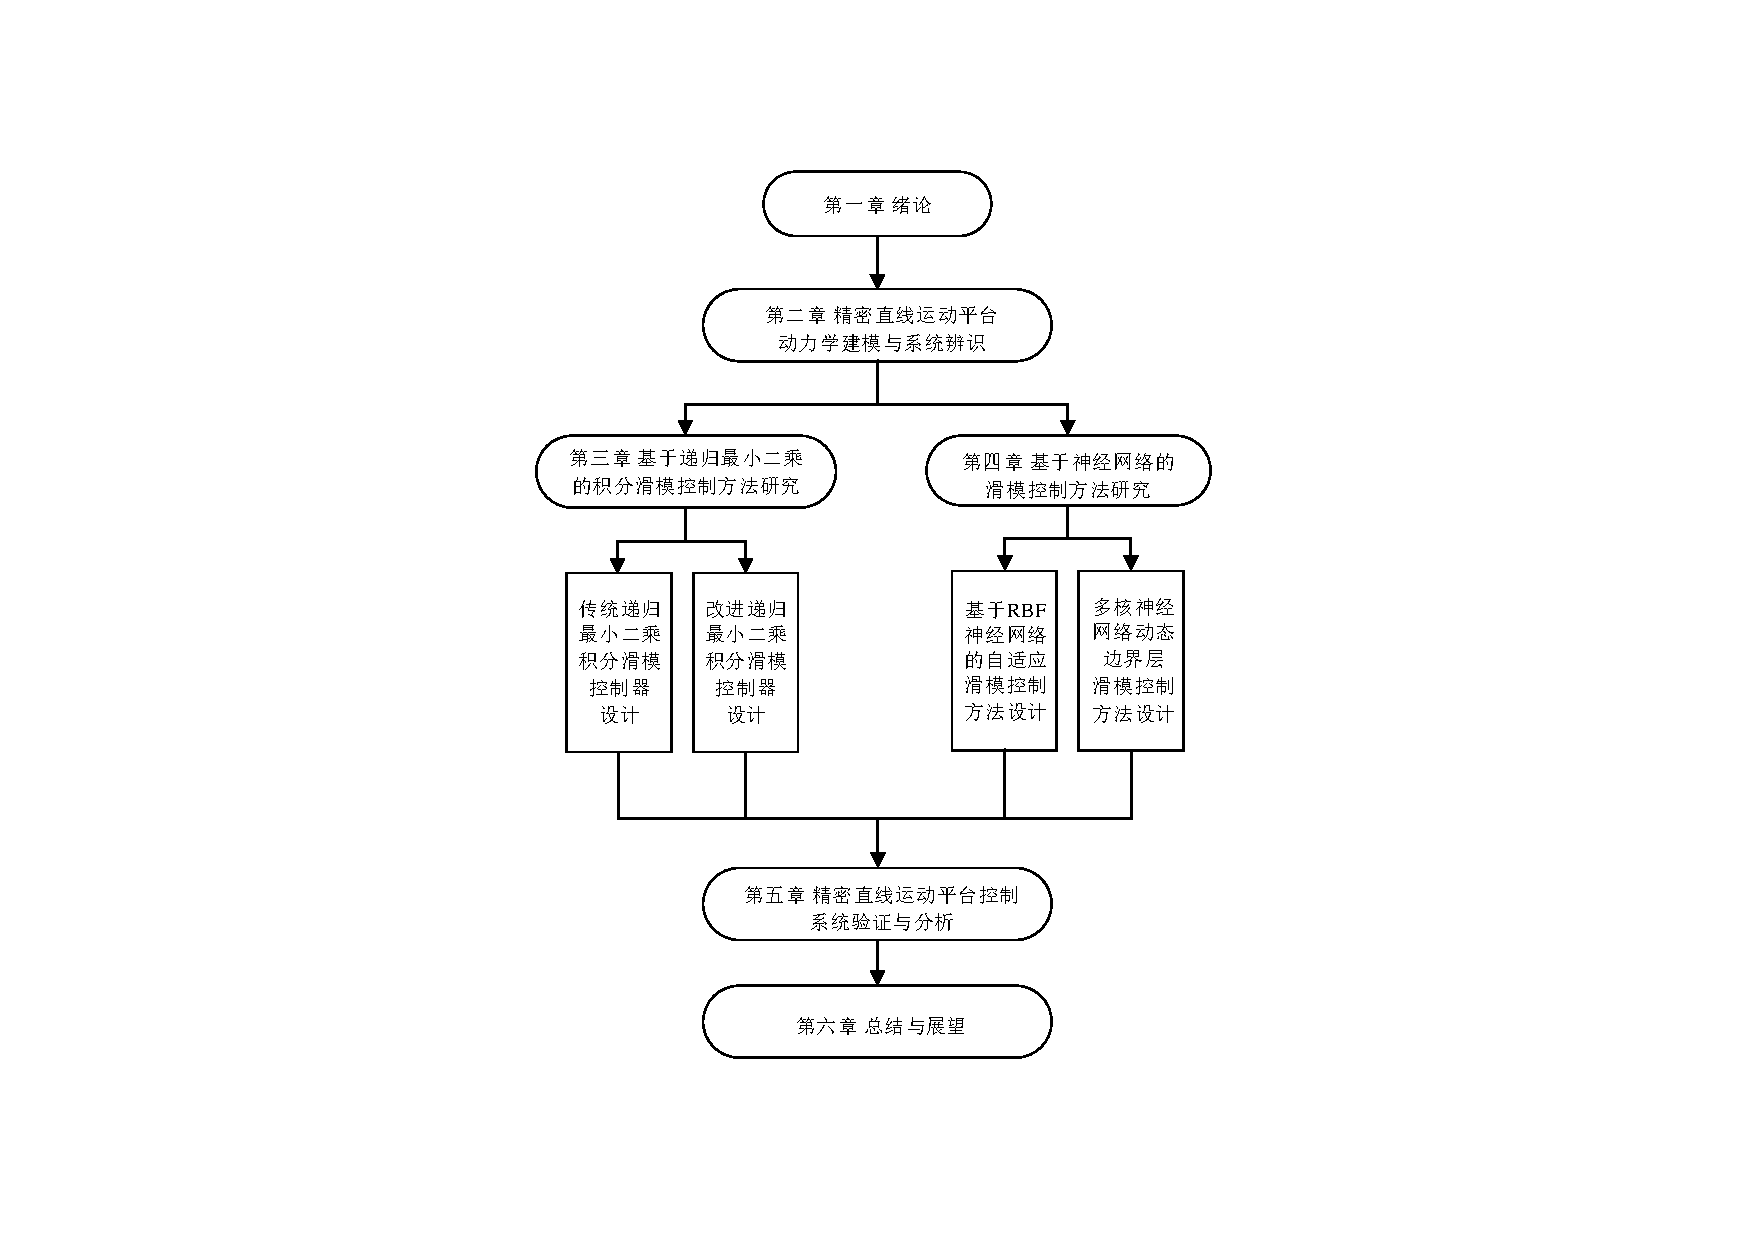
\includegraphics[width=12cm]{figures/章节安排.pdf}
	\caption{论文章节安排}
	\label{论文章节安排}
\end{figure}
